\section{Analysis}

\subsection{Performance in Different Network Scenarios}
\label{sec:performance}

\begin{figure}[H]
\begin{center}
    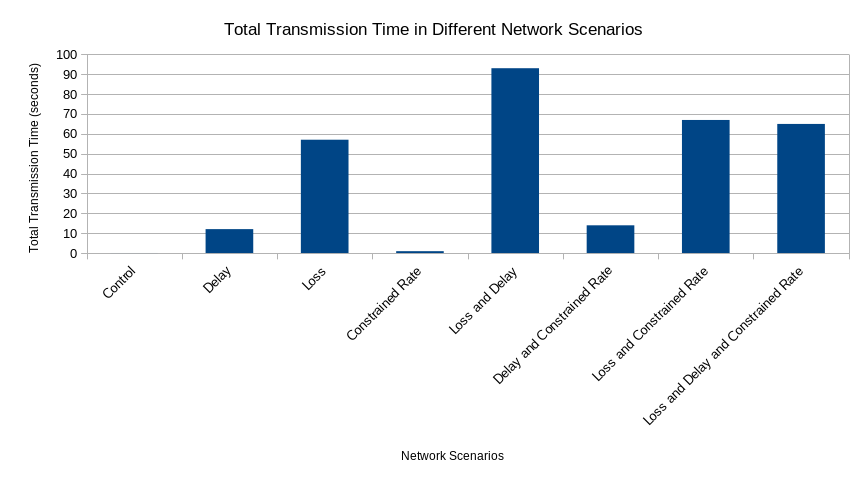
\includegraphics[width=100mm]{images/performance-network-scenarios.png}
\end{center}
\caption{Total Transmission Time in Different Network Scenarios for 230 Kb file.}\label{fig:performance}
\end{figure}

From Figure \ref{fig:performance} we can see that the network characteristic that has the biggest impact on the performance RDT is packet loss. 

\subsection{Bandwidth Delay Product and Link Utilisation}

The Bandwith-Delay Product (BDP) for a link represents the \textbf{what?} and is calculated as:

\begin{align*}
    BDP = \text{Bandwidth (bits per second)} \times \text{Round Trip Time (seconds)}
\end{align*}

For the link between \code{pc7-082-l} and \code{pc7-085-l} the observed average RTT with RDT was \textbf{0.106ms}. This therefore yields a BDP of \textbf{BDP}.

As RDT only sends $1300 \text{\;bytes} = 10400 \text{\;bits}$ in each packet, this means that RDT achieves a link utilisation of $1040 / BDP = $.

\subsection{Maximum Theoretical Data Rate}



\subsection{Idle-RQ Performance}

\begin{align*}
    U_{RDT_IRQ} = \frac{N_pT_x}{T_x + 2T_p}
\end{align*}

where:
\begin{itemize}
    \item $N_p$ is the number of packets sent
    \item $T_x$ is the tranmission delay
    \item $T_p$ is the propogation delay
\end{itemize}

\subsection{RDT Packet Data Size}


\subsection{Wastage due to Control Information}

\begin{align*}
    \rho = \frac{i - c}{i + a} = \frac{1312 - 12}{1312 + 12} = 0.982 \text{\:(3 s.f.)}
\end{align*}